\documentclass[12pt]{article}
\usepackage[utf8]{inputenc}
\usepackage{amsmath}
\usepackage{graphicx}
\usepackage{float}
\setlength{\parindent}{4em}
\setlength{\parskip}{1em}
\renewcommand{\baselinestretch}{1.5}
\title{Intensional infect proportion of newborn, finding eigenvalues}

\begin{document}
\maketitle
\begin{align}
\frac{\mathrm{d}S}{d\tau}&=\epsilon(1-p)- \mathcal{R}_0  SI-\epsilon S \\
\frac{\mathrm{d}I}{d\tau}&=\mathcal{R}_0 SI+\epsilon p-I
\end{align}

Here $\gamma$ is mean infectious period, $\mu$ is birth/death rate, $p$ is probability of intensional infection on newborns. $\epsilon=\frac{\mu}{\gamma+\mu}$,$\mathcal{R}_0$ is the basic reproduction number.
\section{EE}
So to find the E.E. Letting both equal to 0, solve get:
\begin{align}
I &= \frac{\epsilon(\mathcal{R}_0 -1)+ \epsilon \sqrt{(\mathcal{R}_0-1)^2+4\mathcal{R}_0 p}}{2\mathcal{R}_0}\\
S &=\frac{1}{\mathcal{R}_0}-\frac{2p}{(\mathcal{R}_0 -1)+ \sqrt{(\mathcal{R}_0-1)^2+4\mathcal{R}_0 p}}\\
\mathcal{R}_0 I &= \frac{\epsilon(\mathcal{R}_0 -1)+ \epsilon \sqrt{(\mathcal{R}_0-1)^2+4\mathcal{R}_0 p}}{2}\\
\mathcal{R}_0 S &= 1-\frac{2p \mathcal{R}_0}{(\mathcal{R}_0 -1)+ \sqrt{(\mathcal{R}_0-1)^2+4\mathcal{R}_0 p}}
\end{align}

Jacobian is the following.
\begin{equation}
\mathcal{J} =
\begin{bmatrix}
    \ -\mathcal{R}_0 I-\epsilon       & -\mathcal{R}_0 S \\
    \ \mathcal{R}_0 I       & \mathcal{R}_0 S-1 \\
\end{bmatrix}
\end{equation}

Now for simplicity, let $(\mathcal{R}_0 -1)+ \sqrt{(\mathcal{R}_0-1)^2+4\mathcal{R}_0 p}$ = $K$.Notice, $K>0$ if $q\neq 0$

So we get:
\begin{align}
\mathcal{R}_0 I &= \frac{\epsilon K}{2}\\
\mathcal{R}_0 S &= 1-\frac{2p \mathcal{R}_0}{K}
\end{align}

\begin{equation}
\mathcal{J} =
\begin{bmatrix}
    \ -\frac{\epsilon K}{2}-\epsilon       & -1+\frac{2p \mathcal{R}_0}{K} \\
    \ \frac{\epsilon K}{2}       & -\frac{2p \mathcal{R}_0}{K} \\
\end{bmatrix}
\end{equation}

The eigenvalues of this Jacobian is:

\begin{equation}
\lambda = \frac{-(\epsilon K^2+2\epsilon K +4p\mathcal{R}_0) \pm \sqrt{(\epsilon K^2+2\epsilon K +4p\mathcal{R}_0)^2-4(2\epsilon K^3+8\epsilon Kp\mathcal{R}_0)}}{4K}
\end{equation}

Since $\sqrt{(\epsilon K^2+2\epsilon K +4p\mathcal{R}_0)^2-4(2\epsilon K^3+8\epsilon Kp\mathcal{R}_0)}\leq |\epsilon K^2+2\epsilon K +4p\mathcal{R}_0|$, we can conclude that Re($\lambda$)$<0$ for all $p\neq 0$

We are interested in whether this is a damped oscillation or not, so we look into the discriminant.

\subsection{Take $p$ as the variable}

The following values are used: $\mu=\frac{1}{50*365}$, $\gamma=\frac{1}{22}$, $\mathcal{R}_0=4.5$. Also, $\epsilon=\frac{\mu}{\mu+\gamma}=0.0012$

I plotted the discriminant with Mathematica, domain of $p$ is $[0,1]$.

\begin{figure}[H]
  \caption{Plot discriminant with $p$ to be the variable.}
  \centering
  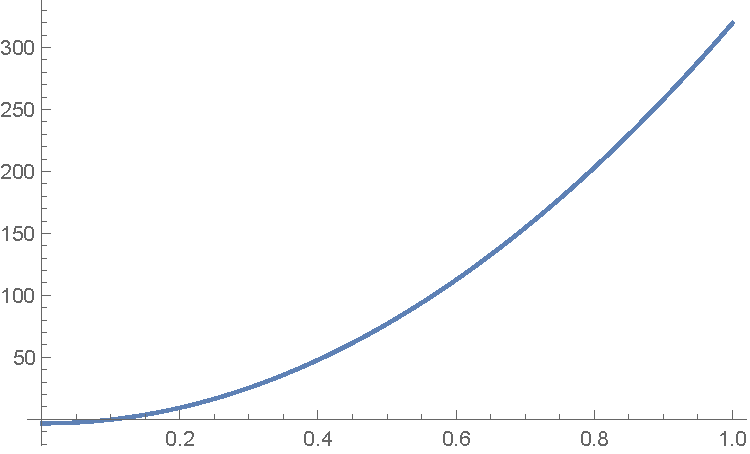
\includegraphics[width=1.1\textwidth]{Figures/Discriminant_plot_newborn.pdf}
\end{figure}

The $p$-intercept of this graph is $p=0.103995$. Meaning, with a proportion of 0.103995 or less, there is going to be a damped oscillation.

\subsection{Take $\mathcal{R}_0$ as the variable}.

This time, I take $\mu=\frac{1}{80*365}$, $\gamma=\frac{1}{22}$, $\epsilon=\frac{\mu}{\mu+\gamma}=0.000753$.

I made a sequence of plots by taking $p=0.1,0.2,0.3...$

\begin{figure}[H]
  \caption{Plot discriminant with $\mathcal{R}_0$ to be the variable.$p=0.1$, the $\mathcal{R}_0$ -intercept is $\mathcal{R}_0 = 0, 5.74966$}
  \centering
  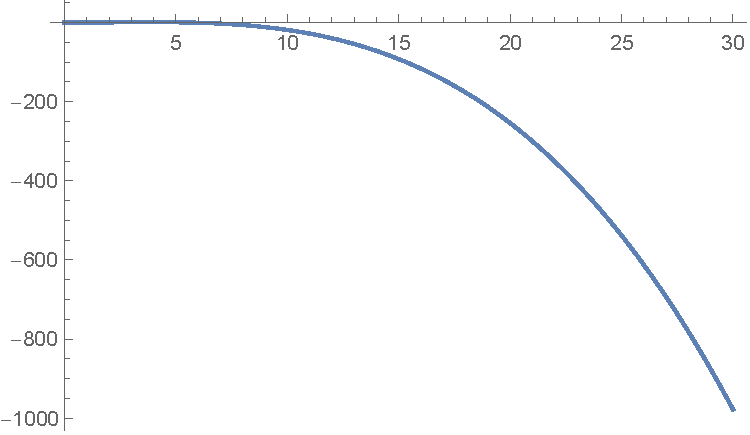
\includegraphics[width=1.1\textwidth]{Figures/Plot_R_0_p_0_1.pdf}
\end{figure}

\begin{figure}[H]
  \caption{Plot discriminant with $\mathcal{R}_0$ to be the variable.$p=0.2$, the $\mathcal{R}_0$ -intercept is $\mathcal{R}_0 = 0, 17.0518$}
  \centering
  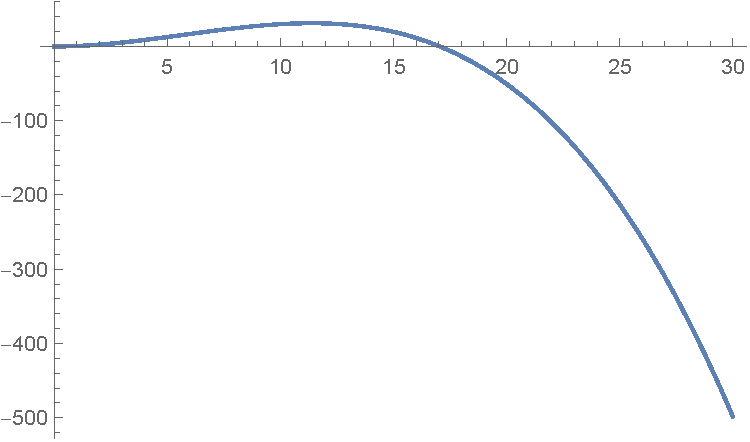
\includegraphics[width=1.1\textwidth]{Figures/Plot_R_0_p_0_2.pdf}
\end{figure}

\begin{figure}[H]
  \caption{Plot discriminant with $\mathcal{R}_0$ to be the variable.$p=0.3$, the $\mathcal{R}_0$ -intercept is $\mathcal{R}_0 = 0, 37.4537$}
  \centering
  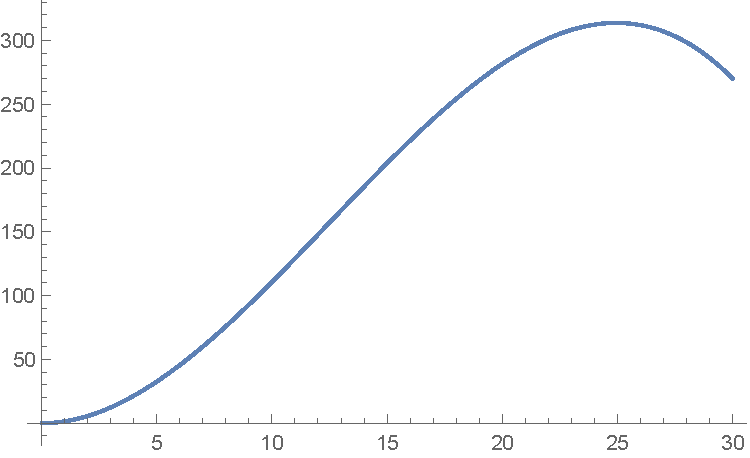
\includegraphics[width=1.1\textwidth]{Figures/Plot_R_0_p_0_3.pdf}
\end{figure}

For $p=0.4$ or higher, the graphs look similar, but with even higher value for the discriminant and larger value for $\mathcal{R}_0$-intercept.

\section{DFE}

Disease free equilibrium is the equilibrium when there is nobody infected in the system, which means, $I=0$

Thus we have $\frac{\mathrm{d}I}{d\tau}=\mathcal{R}_0 SI+\epsilon p-I=\epsilon p=0$

In our case, there is no DFE. When $I=0$, we are still intensionally infecting susceptible,  therefore, there is no equilibrium in which $I=0$.

\end{document}
